\section{Experiments and Evaluation}
\subsection{Environment}
We used the game "Breakout" from the Gym toolkit \cite{brockman2016openai} as an
environment. Breakout is a game in which the player controls a paddle to bounce the ball and destroy blocks. The player wins if no block is left, but loses if the ball is dropped.

The RL agent learning and playing the game was Proximal
Policy Optimization (PPO) \cite{raffin2019stable}. PPO is an on-policy
algorithm, that uses an actor critic approach. We started with the stablebaselines3 implementation \cite{raffin2019stable}, and
modified it to our needs.

\subsection{Dimension reduction}\label{sub:Dimension_reduction}
Our first experiments featured the basic dimension reduction method,
without the modifications for compression. The goal was to verify the
required reconstruction information was present within the feature extractor's lower dimensional
representation. The qualitative results can be
seen in Figure \ref{fig:baseline_MSE} (Note: images came
from training set). \\

\begin{figure}[H]
    \centering
    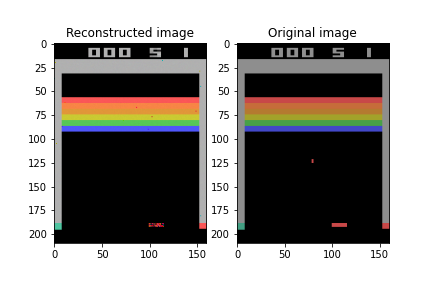
\includegraphics[width=\linewidth]{images/orig_reconstructed0.0.png}
    \caption{Baseline method (no compression) with decoder trained on MSE for 10,000 iterations}
    \label{fig:baseline_MSE}
\end{figure}


\subsection{Compression}\label{sub:Results_Compression} Now we added the
compression loss to the RL agent training, equation \ref{eq:RL_Training_Loss}
and trained the agent with this loss function. We modified the $\alpha$ value,
looking at the performance of the decoder after some epochs. An $\alpha$ of
$1e-4$ worked best, therefore we chose this value for an extended run over $1e5$
epochs. Tested on an independently created test dataset, this resulted in an
entropy of 1.7 bits per latent dimension, when the latent values were rounded to
3 digits. The actual bitrate given by the cross-entropy \ref{eq:BitRate} is
higher however, as we must choose a fixed latent encoding and transmission
distribution. For training we chose a Normal distribution with mean 0 and
learned variance, also used for testing. The expected variance per dimension was
estimated by the mean per dimension over the whole test dataset. However, the
test cross-entropy was significantly higher, mostly in the order of at least
times 1000. A visual investigation of the latent values showed that while the
entropy of the latent values was low, some values deviated from 0 significantly
in the order of 100, leading to a probability of nearly 0.

After training the RL Agent, the decoder was trained for $2e5$ epochs. This
resulted in an MSE Loss of 1895. As discussed in \ref{sec:Introduction}, MSE
is an unideal metric for performance, since it gives each pixel the same
value. Therefore we investigated some images qualitatively. An example can be seen in figure
\ref{fig:final_agent}.
\begin{figure}[H]
    \centering
    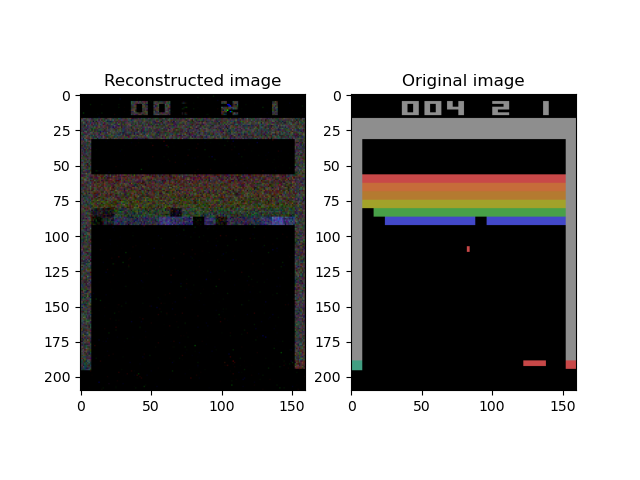
\includegraphics[width=\linewidth]{images/orig_reconstructed_final_agent.png}
    \caption{Final agent}
    \label{fig:final_agent}
\end{figure}

\subsection{Latent Loss Scheme}
As discussed in section \ref{sec:Introduction}, $L_2$ Loss may be suboptimal and
we introduced a latent loss scheme \ref{sub:Distortion} as an alternative.
Training a decoder with the latent loss scheme showed an image quality decrease
compared to $L_2$ Loss, (see figure \ref{fig:baseline_MSE_latent}) (also from
the training set).

\begin{figure}[H]
    \centering
    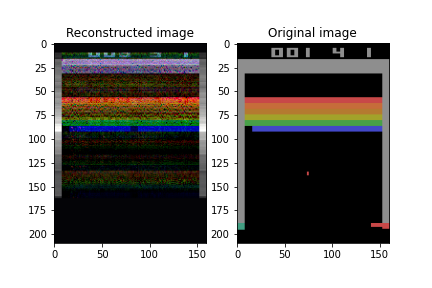
\includegraphics[width=\linewidth]{images/orig_reconstructed_rl3.0.png}
    \caption{Baseline method (no compression) with decoder trained on MSE for 10,000 iterations, then latent MSE for 10,000 iterations}
    \label{fig:baseline_MSE_latent}
\end{figure}

\subsection{Adaptive Alpha}
When implementing our custom loss function with static $\alpha$, several
rudimentary tests were performed to verify the model behaved as expected. One
such test involved varying $\alpha$: we expected that a lower value would
prioritize task performance, while a higher value would prefer a lower bitrate.
However, we found this was not the case: there seemed to be just as much
variation between independent tests of the same $\alpha$ as changing $\alpha$.
Given our hypothesis for where the problem lay (see \ref{sub:Adaptive_Alpha}),
we developed the adaptive $\alpha$ scheme. However, initial results showed no
improvement and this was moved to Future Work.

\subsection{Pretrained agents}
Another idea was that adding the compression loss to the RL agent from the
beginning on was too large of a constraint for the agent to learn anything.
Therefore, we tried to fix this by pretraining the agent before adding
the compression loss to the agent. On the one hand, the additional compression
loss reduced the entropy but on the other hand, the decoder did not learn
after the training, so this procedure showed no improvements.


